Dialog \glqq{}Hauptmenü\grqq{}

Im Hauptmenü kann der Benutzer über den Spielen-Button in die Lobby-Übersicht gelangen, wenn die Verbindung erfolgreich aufgebaut werden konnte. Falls nicht, erscheint eine Fehlermeldung als Popup. Mit dem Button Einstellungen kommt der Benutzer zu dem Einstellungen-Dialog. Durch Klick auf den Hilfe-Button öffnet sich ein Popup, in dem dem Nutzer hilfreiche Informationen zur Verfügung gestellt werden. Mit dem Beenden-Button kann der Benutzer die Anwendung verlassen und schließen.

\begin{figure}
  \centering
  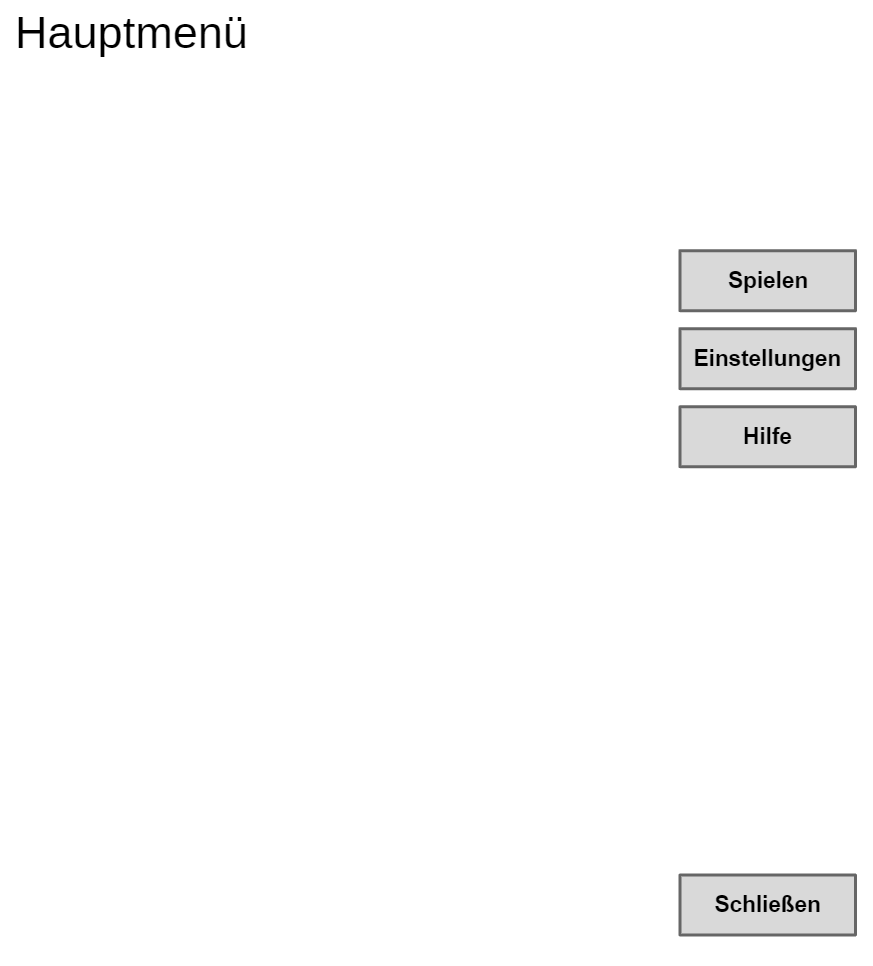
\includegraphics[width=\textwidth]{Meilenstein03/Hauptmenue_Mockup.png}
  \caption{Mockup für das Hauptmenü}
\end{figure}

Dialog \glqq{}Einstellungen\grqq{}

In den Einstellungen kann man diverse Einstellungen vornehmen. Über den Button Hauptmenü gelangt man zurück ins Hauptmenü.

\begin{figure}
  \centering
  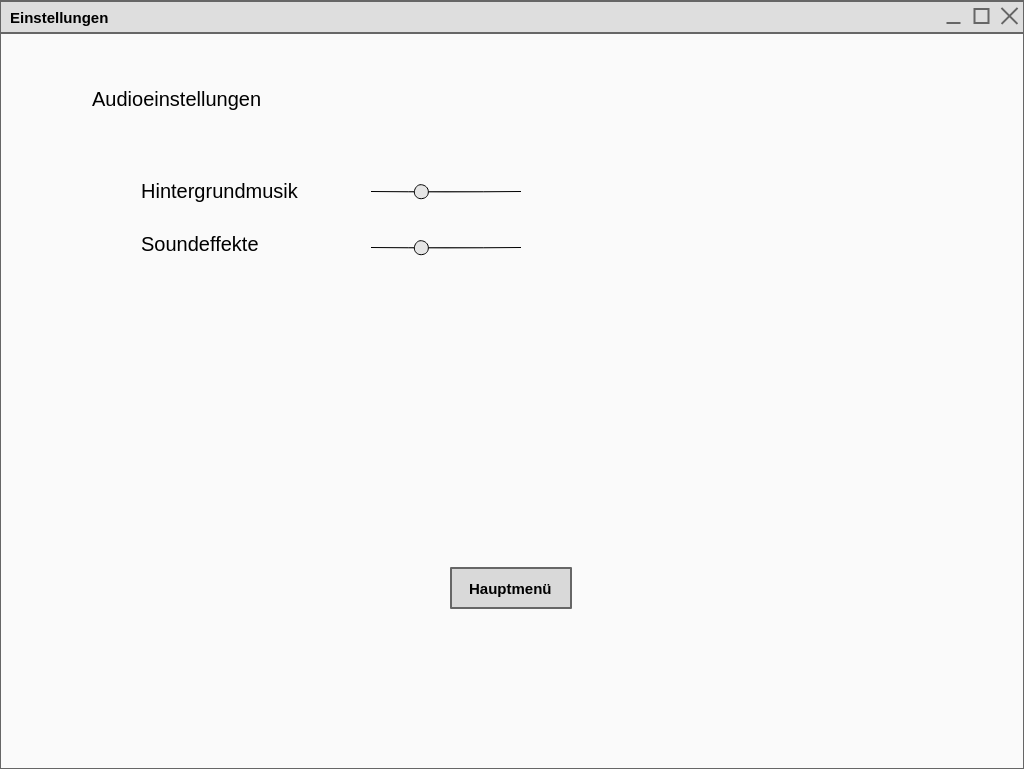
\includegraphics[width=\textwidth]{Meilenstein03/Einstellungen_Mockup.png}
  \caption{Mockup für die Einstellungen}
\end{figure}

Popup \glqq{}Hilfe-Hauptmenü\grqq{}

In dem Hilfe-Popup werden dem Benutzer alle möglichen Interaktionen mit dem entsprechenden Dialog aufgezeigt.

\begin{figure}
  \centering
  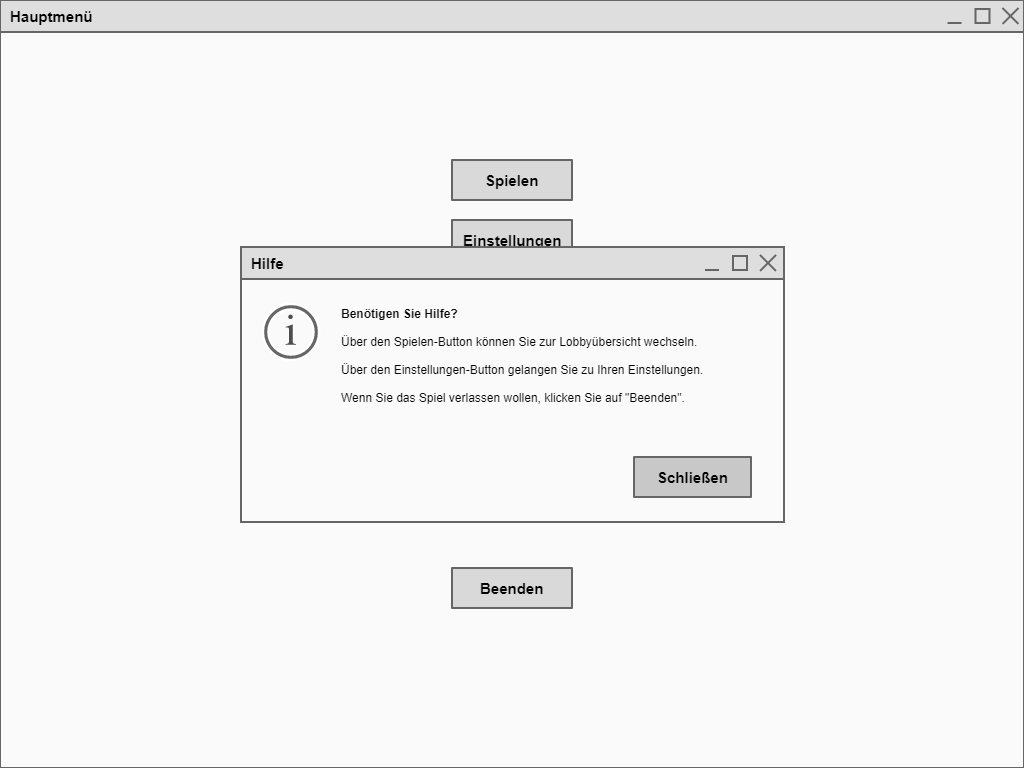
\includegraphics[width=\textwidth]{Meilenstein03/Hilfe-Hauptmenue_Mockup.png}
  \caption{Mockup für das Hilfe-Hauptmenü-Popup}
\end{figure}

Popup \glqq{}Fehler bei der Verbindung zum Server\grqq{}

Falls die Verbindung zum Server fehlgeschlagen ist, wird dem Benutzer ein Popup angezeigt, das ihm diese Information mitteilt.

\begin{figure}
  \centering
  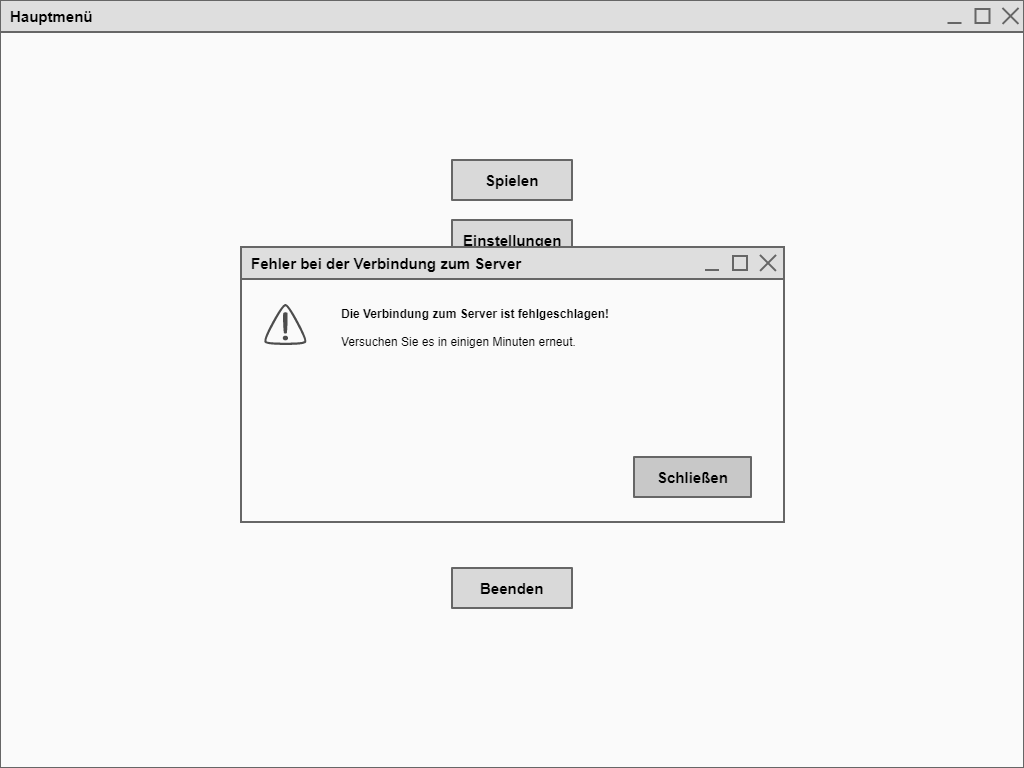
\includegraphics[width=\textwidth]{Meilenstein03/FehlerBeiDerVerbindungZumServer_Mockup.png}
  \caption{Mockup für das Fehler bei der Verbindung zum Server-Popup}
\end{figure}

Dialog \glqq{}Lobby-Übersicht\grqq{}

In der Lobby-Übersicht werden dem Benutzer alle vorhandenen Lobbys und die Anzahl der Spieler und Zuschauer, die sich in ihr befinden, angezeigt. Durch Klicken auf Beitreten kann der Benutzer einer bestehenden Lobby beitreten. Durch Klicken auf den Verlassen-Button gelangt man zum Hauptmenü. Der Aktualisieren-Button aktualisiert die Lobby-Übersicht. Mit dem Button Namen ändern, kann man den Namen einer Lobby verändern. Mit dem Button Lobby erstellen kann man eine neue Lobby erstellen.

\begin{figure}
  \centering
  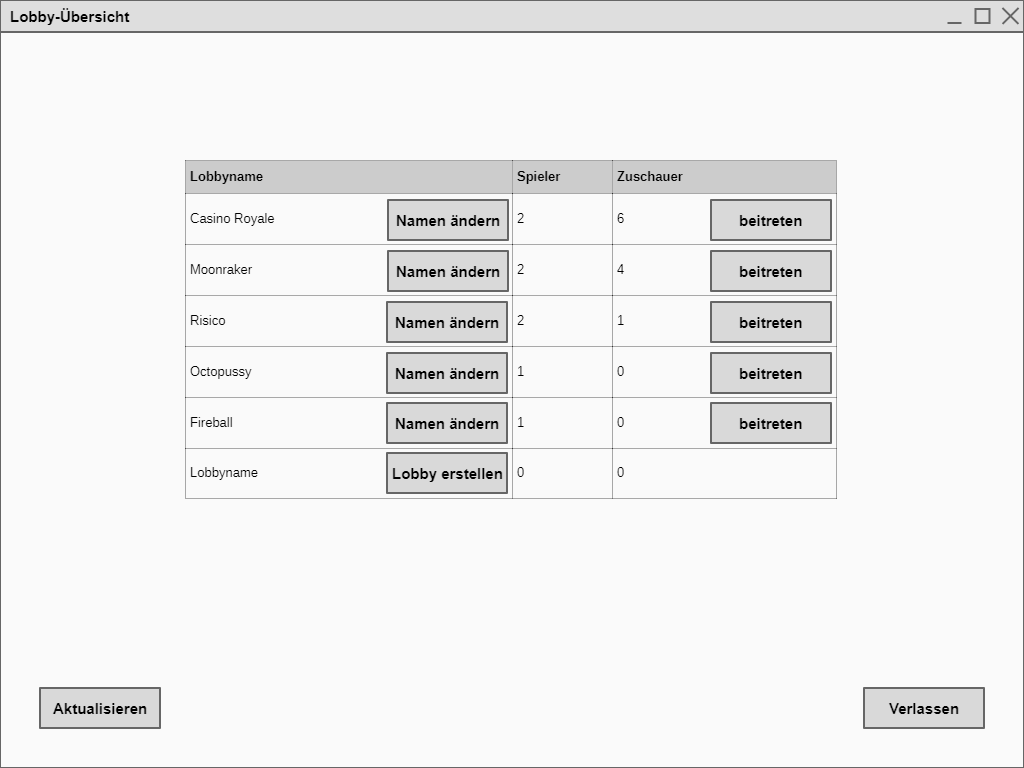
\includegraphics[width=\textwidth]{Meilenstein03/Lobby-Uebersicht_Mockup.png}
  \caption{Mockup für die Lobby-Übersicht}
\end{figure}

Popup \glqq{}Namen ändern\grqq{}

In diesem Popup kann der Benutzer den Namen einer Lobby nachträglich verändern. Durch den Schließen-Button verschwindet das Popup-Fenster und der Benutzer gelangt zurück in die Lobby-Übersicht.

\begin{figure}
  \centering
  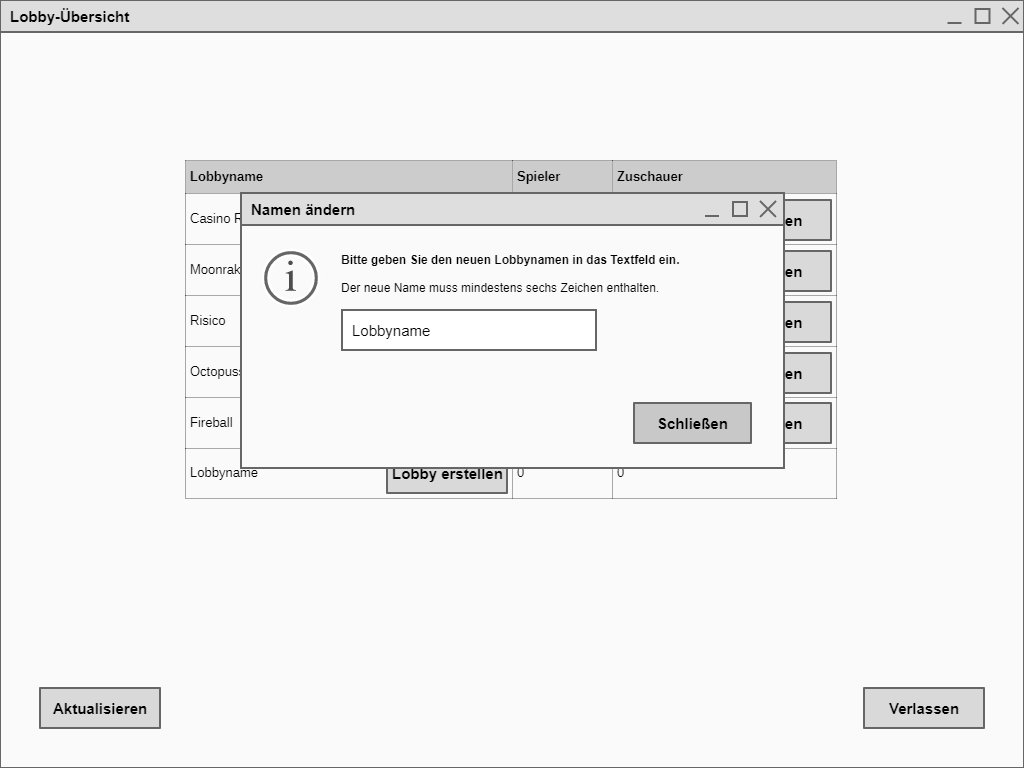
\includegraphics[width=\textwidth]{Meilenstein03/NamenAendern_Mockup.png}
  \caption{Mockup für das Namen ändern-Popup}
\end{figure}

Popup \glqq{}Lobbynamen eingeben und Konfig. erstellen\grqq{}

In diesem Popup kann der Benutzer eine neue Lobby erstellen. Dazu muss er den Lobbynamen und eine Konfiguration festlegen. Durch Klicken auf den Button Neue Konfig. kann der Benutzer eine Konfiguration auswählen oder eine Neue erstellen. Durch Klicken auf den Bestätigen-Button, kommt der Benutzer zurück in die Lobbyübersicht.

\begin{figure}
  \centering
  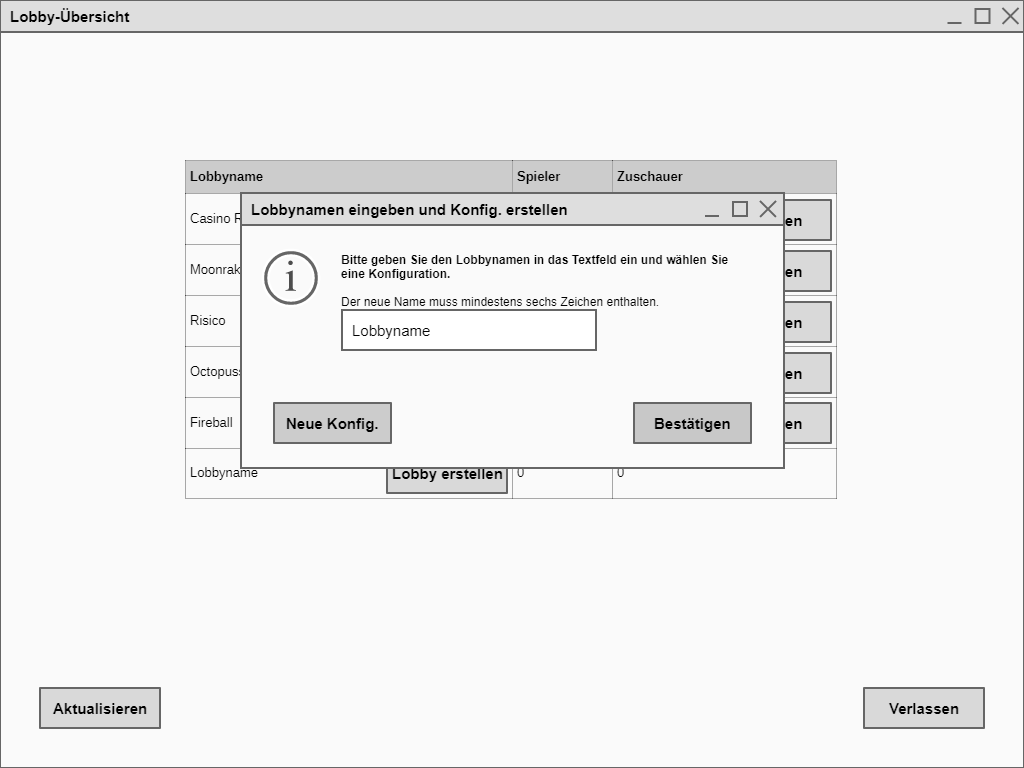
\includegraphics[width=\textwidth]{Meilenstein03/LobbynamenEingebenUndKonfigErstellen_Mockup.png}
  \caption{Mockup für das Lobbynamen eingeben und Konfig. erstellen-Popup}
\end{figure}

Dialog \glqq{}Editor\grqq{}

Mit der Schaltfläche \glqq{}Schließen\grqq{} wechselt man zum Dialog \glqq{}Lobby-Übersicht\grqq{}.
Mit der Schaltfläche \glqq{}Hilfe\grqq{} öffnet sich ein Hilfe-Popup, in dem dem Benutzer Informationen zu möglichen Interaktionen angezeigt werden.
In den drei Dropdown-Menüs kann der Benutzer das gewünschte Szenario, die gewünschte Charakterliste und die gewünschte Partie-Konfiguration auswählen. Wenn man in einem Dropdown-Menü den Eintrag 'Neue(s) Szenario/Charakterliste/Partie-Konfiguration erstellen' auswählt, dann wechselt die Ansicht zum Dialog \glqq{}Szenario-/Charakter-/Partie-Editor\grqq{} und eine neue Datei des entsprechenden Typs wird erstellt und zum Editieren geöffnet.
Wenn man in einem der Dropdown-Menüs einen Eintrag auswählt, dann wird eine Schaltfläche mit der Aufschrift \glqq{}bearbeiten\grqq{} neben dem Eintrag angezeigt. Mit dieser Schaltfläche wechselt man ebenfalls in den entsprechenden Editor und die Datei des Eintrags wird geöffnet zum Editieren.

\begin{figure}
  \centering
  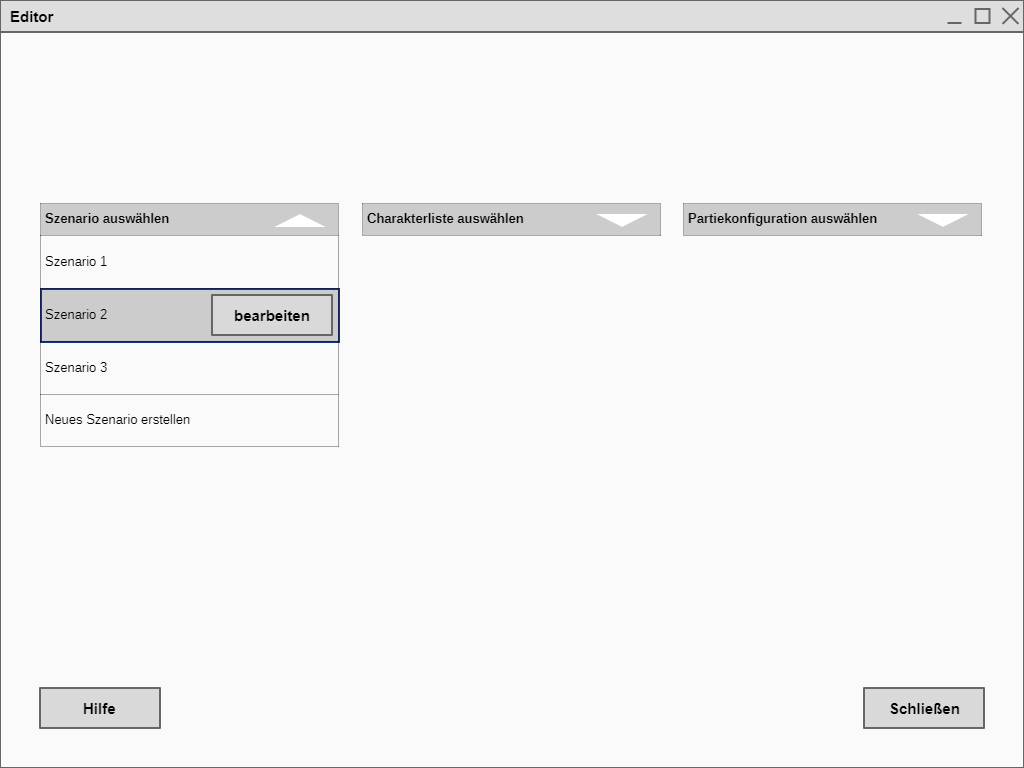
\includegraphics[width=\textwidth]{Meilenstein03/Editor_Mockup.png}
  \caption{Mockup für den Editor}
\end{figure}

Popup \glqq{}Hilfe-Editor\grqq{}

In diesem Popup wird dem Benutzer mitgeteilt, welche Interaktionen er mit dem Editor-View eingehen kann. Über den Schließen-Button wird das Hilfe-Popup-Fenster geschlossen und der benutzer kehrt zum Editor zurück.

\begin{figure}
  \centering
  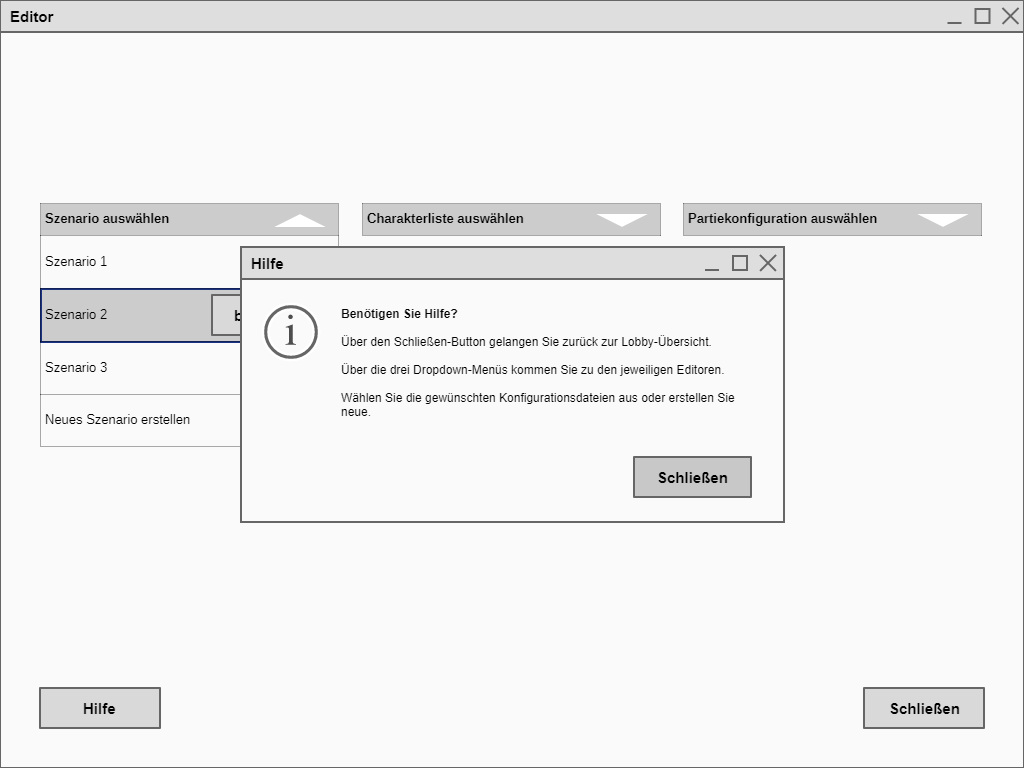
\includegraphics[width=\textwidth]{Meilenstein03/Hilfe-Editor_Mockup.png}
  \caption{Mockup für das Hilfe-Editor-Popup}
\end{figure}

Dialog \glqq{}Lobby\grqq{}

Die Liste mit den verbundenen Clients wird kontinuierlich sortiert, sodass die Spieler immer an oberster Stelle stehen. Die Spieler und die Zuschauer werden untereinander chronologisch nach Beitritt zur Lobby bzw. dem letzten Rollenwechsel sortiert, sodass der Client, der als letzter als Zuschauer der Lobby beigetreten ist bzw. als letzter innerhalb der Lobby die Rolle zu Zuschauer geändert hat, den untersten Eintrag in der Liste hat. Die KI-Clients sind am Benutzernamen erkennbar. 
Mit der Schaltfläche \glqq{}Rolle wechseln\grqq{} ändert sich die eigene Rolle von 'Spieler' zu 'Zuschauer' und umgekehrt. 
Mit der Schaltfläche \glqq{}KI hinzufügen\grqq{} wechselt der Client in den Dialog \glqq{}KI-Konfiguration\grqq{}.
Mit der Schaltfläche \glqq{}Zurück\grqq{} wechselt der Client in den Dialog \glqq{}Lobby-Übersicht\grqq{}.
Die Schaltfläche \glqq{}Bereit\grqq{} ist nur für Clients in der Rolle 'Spieler' eingeblendet. Mit dieser Schaltfläche signalisiert der Benutzer, dass er bereit ist, die Spielpartie zu beginnen. Wenn die Schaltfläche gedrückt wird, wird sie ersetzt durch eine Schaltfläche mit der Aufschrift \glqq{}Nicht mehr bereit\grqq{}. Mit dieser Schaltfläche signalisiert der Benutzer, dass er nun doch nicht mehr bereit ist, die Spielpartie zu beginnen. Die Schaltfläche \glqq{}Spiel starten\grqq{} kann nur dann von einem Client gedrückt werden, wenn dieser Client die Rolle 'Spieler' hat und alle Spieler-Clients der Lobby ihre Spielbereitschaft mit Drücken der Schaltfläche \glqq{}Bereit\grqq{} signalisiert haben.
Mit der Schaltfläche \glqq{}Spiel starten\grqq{} wird eine Spielpartie gestartet und die Ansicht wird zum Dialog \glqq{}Spielfeld\grqq{} gewechselt.

\begin{figure}
  \centering
  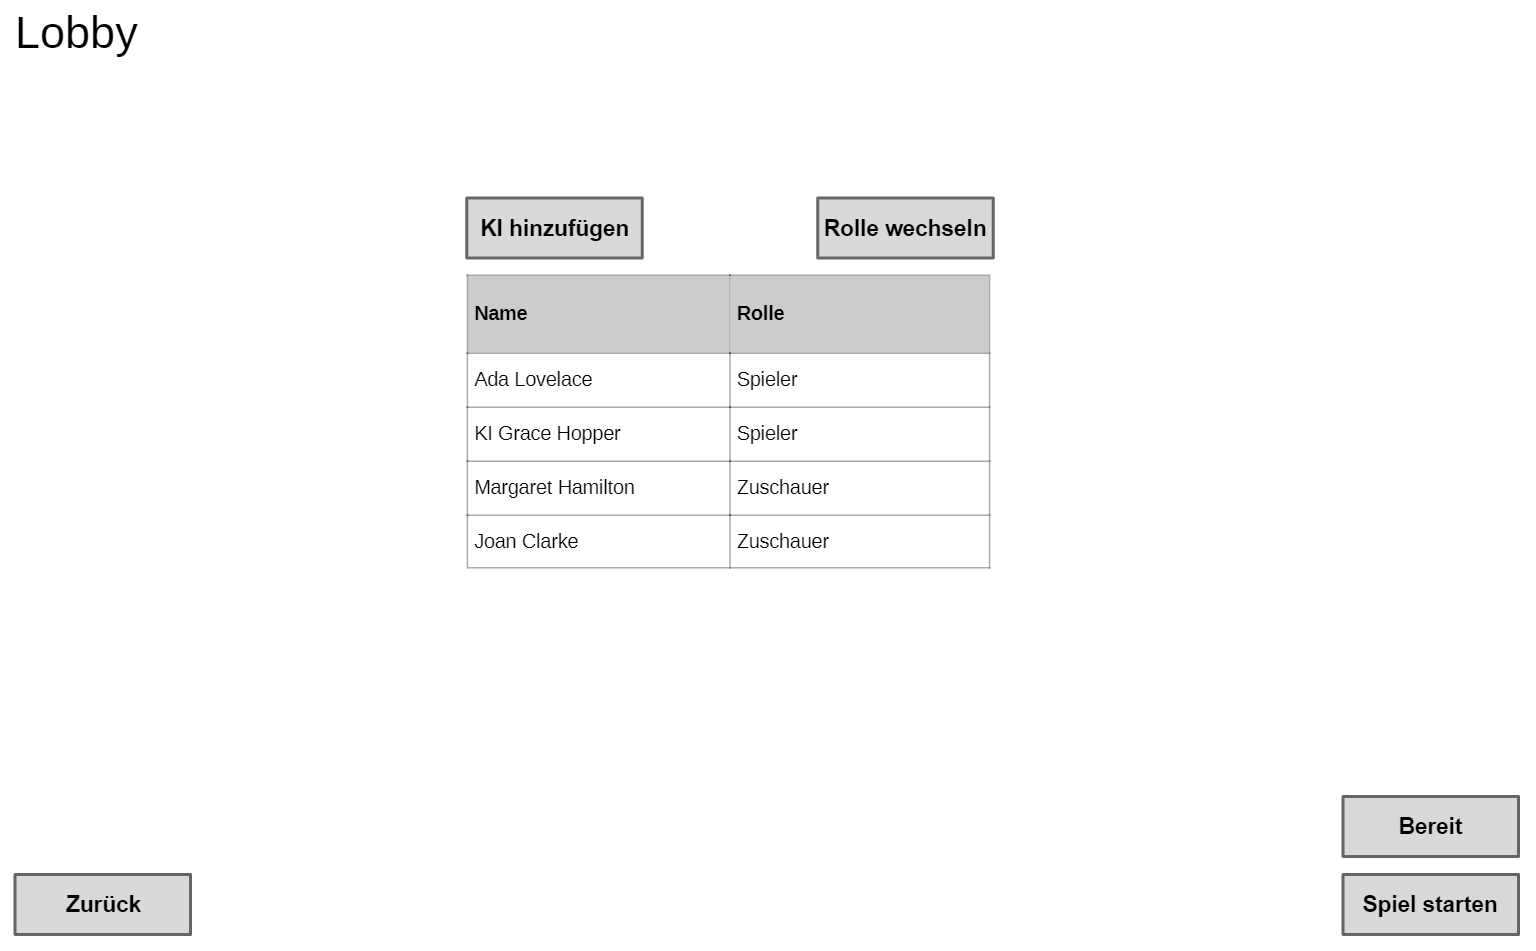
\includegraphics[width=\textwidth]{Meilenstein03/Lobby_Mockup.png}
  \caption{Mockup für das Lobby-View}
\end{figure}

Dialog \glqq{}Szenario-Editor\grqq{}

Alle quadratischen Felder des Spielbretts sind per Mausklick auswählbar. Die Schaltflächen in Form eines Pluszeichens, die den Rand des Spielbretts säumen erweitern das Spielbrett. Wenn eine Plus-Schaltfläche geklickt wird, dann wird sie ersetzt mit einem neuen Feld und an dessen äußeren Rändern, dem neuen äußeren Rand des Spielbretts erscheinen neue Plus-Schaltflächen. Alle Felder des Spielbretts sind zu Beginn freie Felder. Oberhalb des Spielbretts befinden sich die Icons der verschiedenen Feldarten. Diese lassen sich per Drag-and-Drop auf freie Felder des Spielbretts ziehen. Ist die Szenario-Konfiguration abgeschlossen, kehrt der Benutzer über den Speichern-Button auf die letzte Seite zurück. Über den Abbrechen-Button kehrt der Benutzer auch zur letzten Seite zurück und die Änderungen werden verworfen. Über den Editor-Übersicht-Button gelangt der Benutzer zur Editor-Übersicht. Klickt der Benutzer auf den Abbrechen-Button oder auf den Editor-Übersicht-Button, erscheint eine Warnmeldung, die den Benutzer darauf hinweist, dass nicht gespeicherte Änderungen verworfen werden.

\begin{figure}
  \centering
  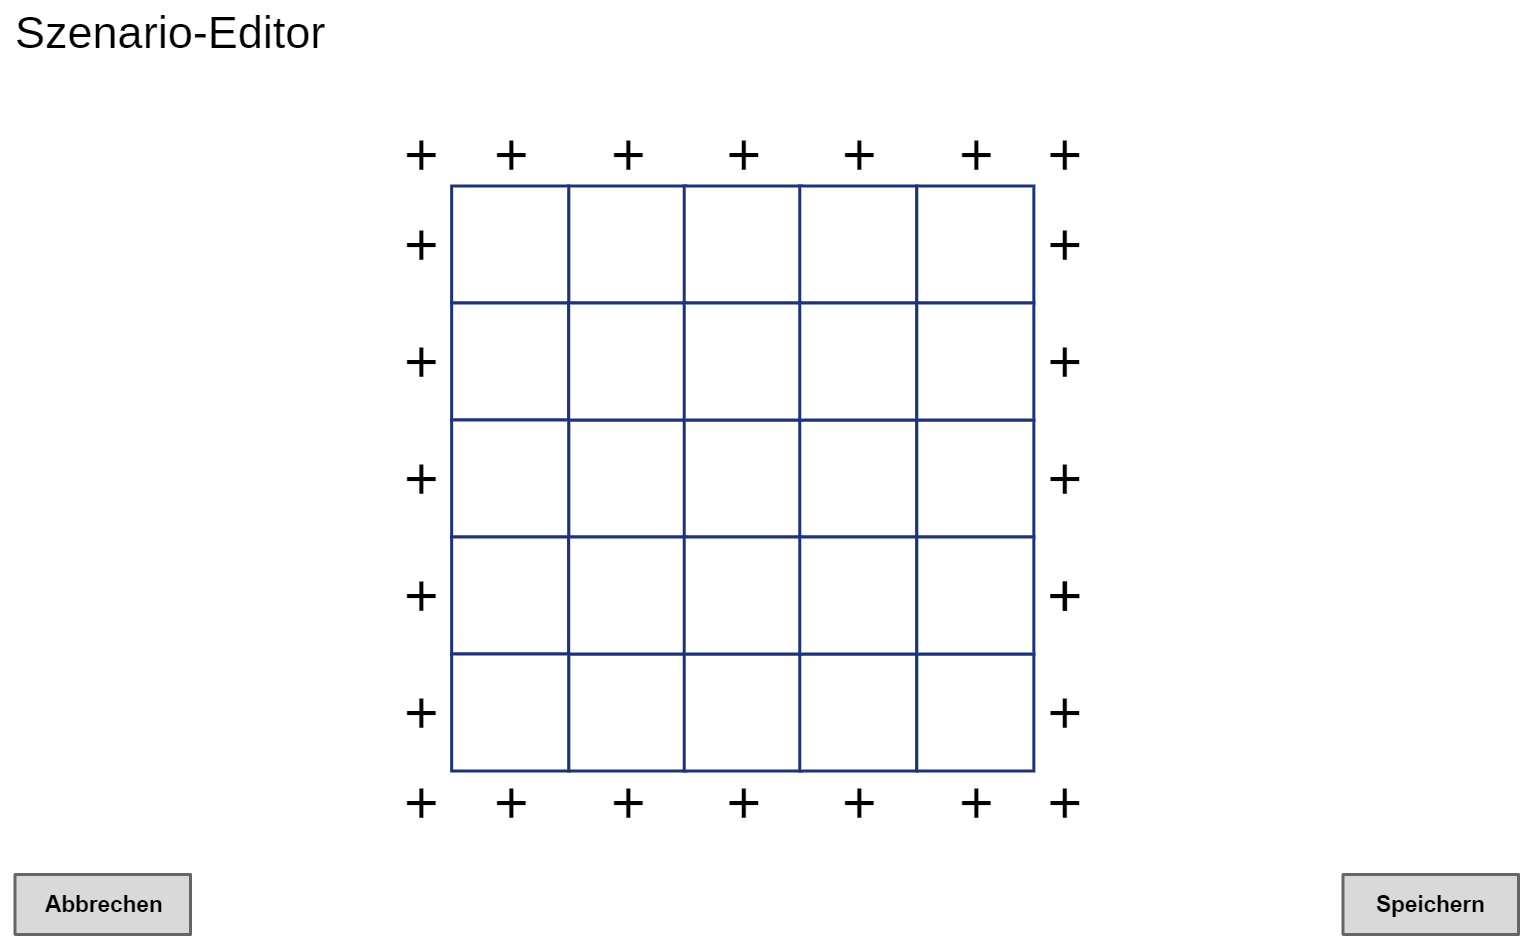
\includegraphics[width=\textwidth]{Meilenstein03/Szenario-Editor_Mockup.png}
  \caption{Mockup für den Szenario-Editor}
\end{figure}

Dialog \glqq{}Charakter-Editor\grqq{}

Dialog \glqq{}Partie-Editor\grqq{}

Mit der Schaltfläche \glqq{}Abbrechen\grqq{} wechselt die Ansicht zu dem Dialog, aus welchem der Partie-Editor aufgerufen wurde. D.h. wenn er aus der Lobby-Konfiguration aufgerufen wurde, dann wechselt die Ansicht zurück zur Lobby-Konfiguration, wenn er aus der Editor-Übersicht geöffnet wurde, dann wechselt die Ansicht wieder dahin zurück.
Mit der Schaltfläche \glqq{}Konfiguration speichern\grqq{} wird die Datei gespeichert und die Ansicht wechselt zu dem Dialog,  aus welchem der Partie-Editor aufgerufen wurde.
Mit der Schaltfläche \glqq{}Editor-Übersicht\grqq{} wird die Ansicht zum Dialog \glqq{}Editor-Übersicht\grqq{} gewechselt, falls alle Änderungen schon gespeichert wurden. Falls noch ungespeicherte Änderungen vorliegen, wird ein Pop-Up-Fenster geöffnet, das abfragt, ob die Konfiguration noch gespeichert werden soll. Wenn in diesem Fenster die Schaltfläche \glqq{}Ja\grqq{} bzw.\glqq{}Nein\grqq{} angeklickt wird, dann wechselt die Ansicht zum Dialog \glqq{}Editor-Übersicht\grqq{} und die Konfiguration wird gespeichert bzw. nicht gespeichert. Mit der Schaltfläche \glqq{}Abbrechen\grqq{} schließt sich das Fenster wieder und der Dialog \glqq{}Partie-Editor\grqq{} wird wieder normal dargestellt.
Mit direkter Eingabe in das Feld der Anzeige des Werts einer Wahrscheinlichkeit oder eines anderen Werts, dem Schieberegler daneben oder den Inkrement- und Dekrementschaltflächen kann der Wert einer Wahrscheinlichkeit in Prozent oder ein Schadens-, Reichweiten-, etc. -wert festgelegt und angepasst werden.

\begin{figure}
  \centering
  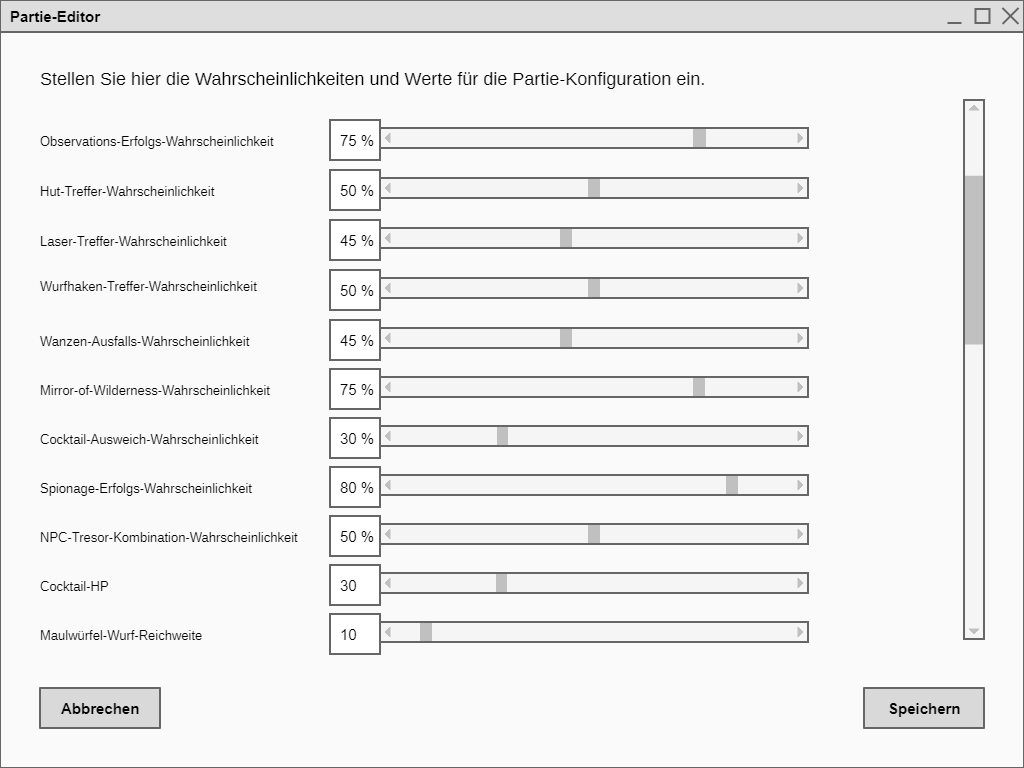
\includegraphics[width=\textwidth]{Meilenstein03/Partie-Editor_Mockup.png}
  \caption{Mockup für den Partie-Editor}
\end{figure}

Dialog \glqq{}KI-Konfiguration\grqq{}

Mit der Schaltfläche \glqq{}Zurück\grqq{} wechselt man zum Dialog \glqq{}Lobby\grqq{}, ohne das ein KI-Client hinzugefügt wurde, mit der Schaltfläche \glqq{}KI hinzufügen\grqq{} wechselt man zum Dialog \glqq{}Lobby\grqq{} und fügt einen KI-Client mit den ausgewählten Parametern hinzu.
Die Intelligenzstufe der KI kann über die Radiobuttons mit den Bezeichnungen 'dumm', 'normal' und 'schlau' eingestellt werden.
Wie in FA-KI 43 beschrieben, muss es möglich sein, die KI mithilfe einer Konfigurationsdatei zu konfigurieren. Deswegen wird in diesem Dialog eine Liste mit Konfigurationsdateien dargestellt, aus denen man eine gespeicherte Konfiguration auswählen kann. Nach der Auswahl einer Konfiguration kann man mit der Schaltfläche \glqq{}Konfiguration laden\grqq{} diese Konfiguration automatisch einstellen.
In das Eingabefeld über der Schaltfläche \glqq{}Konfiguration speichern\grqq{} wird der Name der Konfigurationsdatei vom Benutzer eingetragen. Wenn dort ein valider Dateiname eingegeben wurde, so kann die aktuell eingestellte Konfiguration mit der Schaltfläche \glqq{}Konfiguration speichern\grqq{} in das dafür vorgesehene Verzeichnis gespeichert werden und wird an die Liste der Konfigurationsdateien angefügt.

\begin{figure}
  \centering
  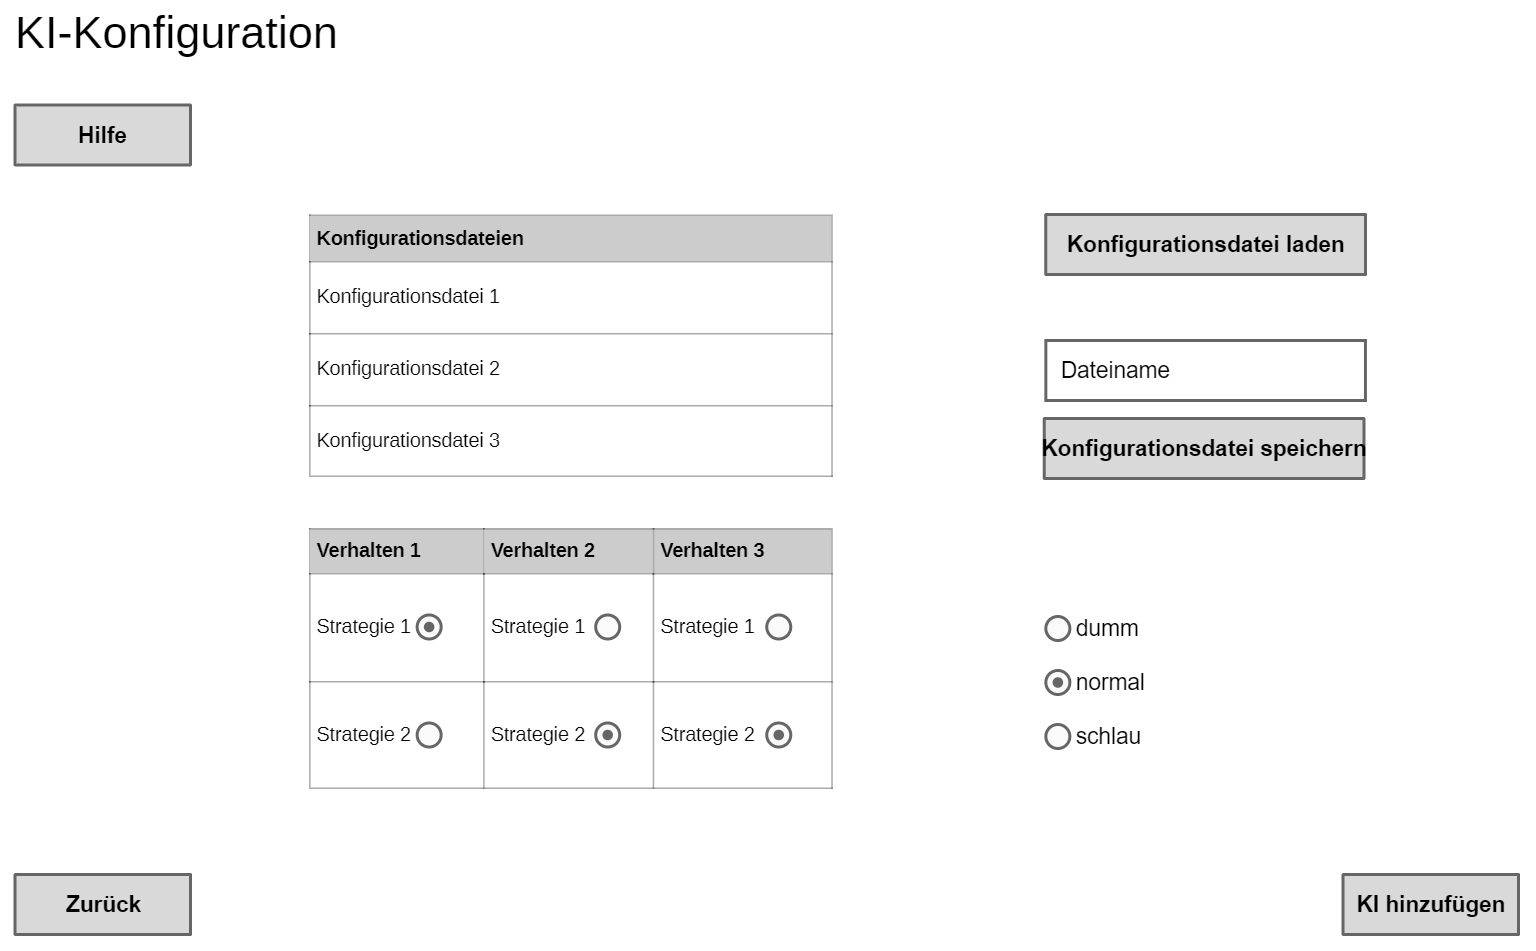
\includegraphics[width=\textwidth]{Meilenstein03/KI-Konfiguration_Mockup.png}
  \caption{Mockup für die KI-Konfiguration}
\end{figure}


\begin{figure}
  \centering
  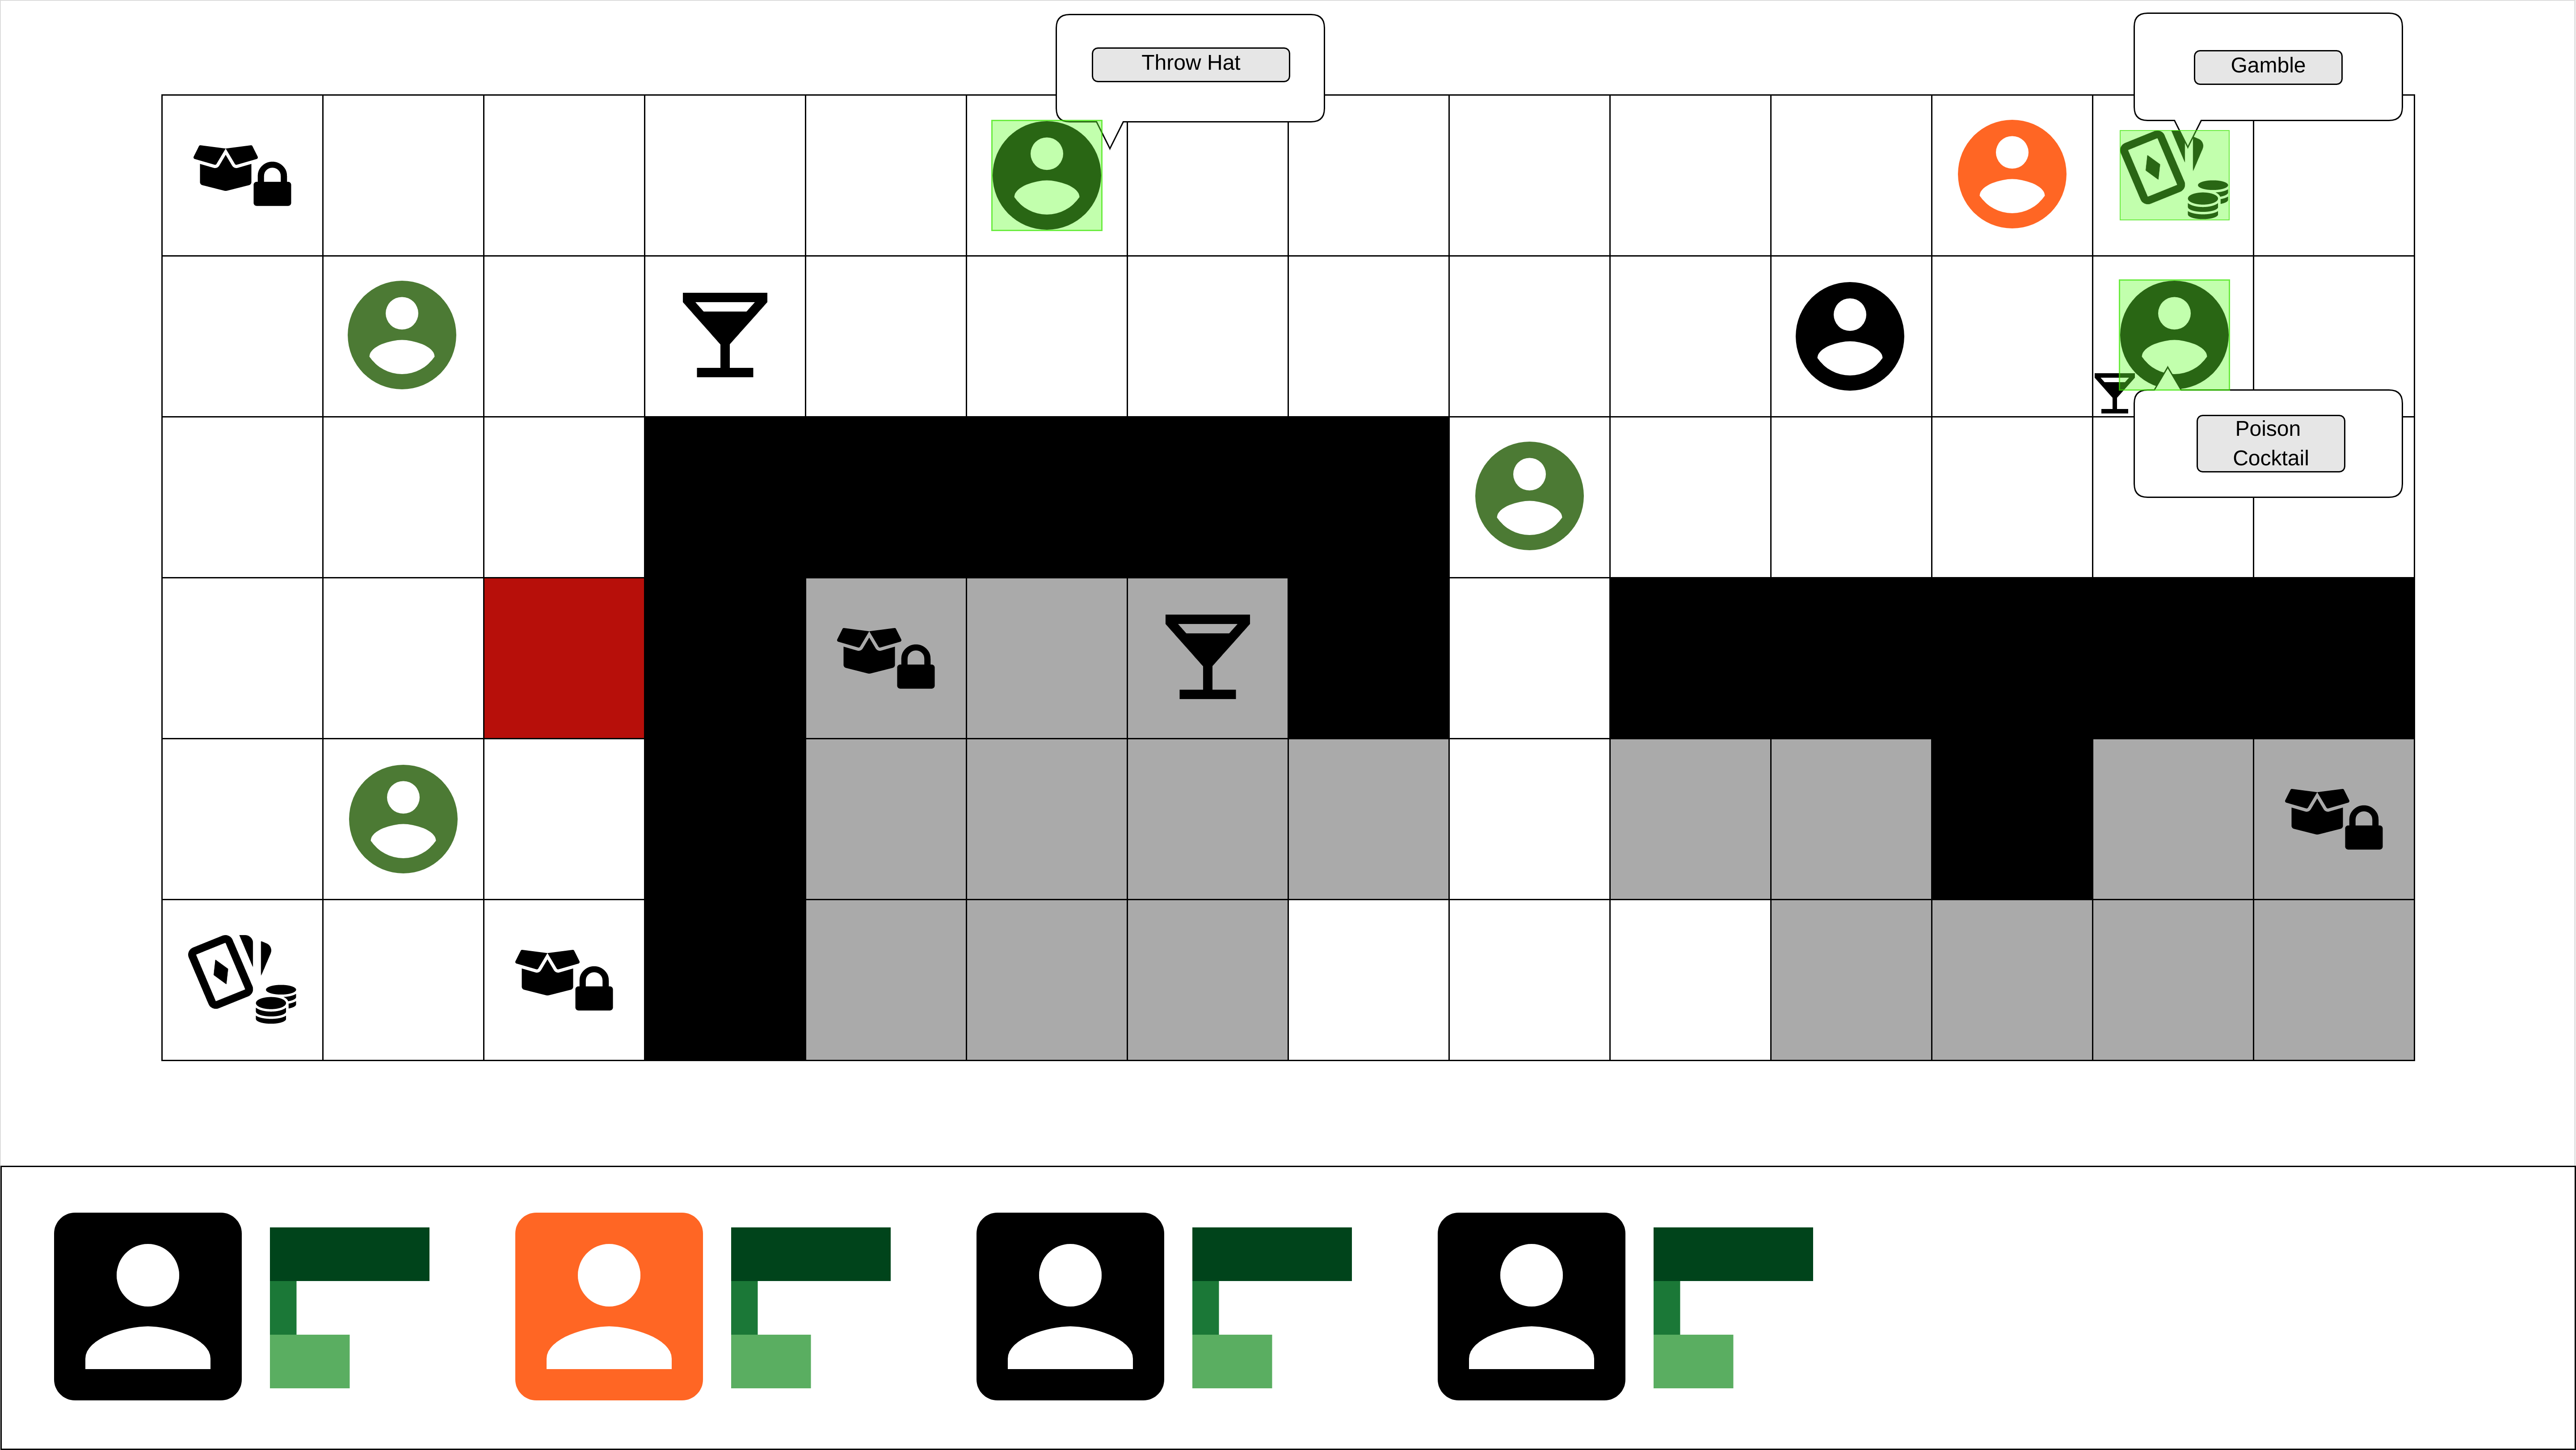
\includegraphics[width=\textwidth]{Meilenstein03/Game_Mockup.png}
  \caption{Mockup für den Spielbildschirm}
\end{figure}
